%%%%%%%% MLSys 2025: LMPool %%%%%%%%%%%%%%%%%

\documentclass{article}

\usepackage{microtype}
\usepackage{graphicx}
\graphicspath{{figures/}}
\usepackage{booktabs}
\usepackage{array}
\usepackage{amsmath}
\usepackage{amssymb}
\usepackage{hyperref}
\urlstyle{same}
\newcommand{\theHalgorithm}{\arabic{algorithm}}

\usepackage[accepted]{mlsys2025}

\makeatletter
\def\subsubsection{\@startsection{subsubsection}{3}{\z@}{-0.08in}{0.01in}
                {\normalsize\bf\raggedright}}
\long\def\@makecaption#1#2{%
  \vskip 10pt
  \baselineskip 11pt
  \setbox\@tempboxa\hbox{{\small #1.} #2}%
  \ifdim \wd\@tempboxa >\hsize
    \sbox{\newcaptionbox}{\small #1.~}%
    \newcaptionboxwid=\wd\newcaptionbox
    \usebox\newcaptionbox {\footnotesize #2}%
  \else
    \centerline{{\small #1.} {\small #2}}%
  \fi}
\makeatother

\newcommand{\sys}{LMPool}
\newcolumntype{L}[1]{>{\raggedright\arraybackslash}p{#1}}

\mlsystitlerunning{LMPool: Locality-Aware Routing and NVLink KV-Cache Transfer}

\begin{document}

\twocolumn[
\mlsystitle{LMPool: Locality-Aware Routing and NVLink KV-Cache Transfer for Multi-GPU LLM Serving}

\begin{mlsysauthorlist}
\mlsysauthor{Jialiang Li}{HKUST}
\end{mlsysauthorlist}

\mlsysaffiliation{HKUST}{The Hong Kong University of Science and Technology}
\mlsyscorrespondingauthor{Jialiang Li}{jl.li@connect.ust.hk}

\mlsyskeywords{Large Language Models, KV Cache, Prefix Caching, Multi-GPU Serving, NVLink}

\vskip 0.3in

\begin{abstract}
Prefix caching avoids repeated prefill computation, but conventional data-parallel LLM replicas manage their KV caches independently. A cache hit may therefore exist on the wrong GPU, while blindly following cache ownership can create a compute hotspot. Moving every reusable prefix is also counterproductive when transfer costs exceed the saved prefill work. We present \sys{}, a Mini-vLLM-based prototype guided by two principles. KV-aware routing addresses cache locality by sending a request to a directly connected GPU that owns the longest useful prefix when the reuse benefit exceeds queue and capacity pressure. NVLink KV transfer provides cache fluidity by copying or moving blocks when cache placement and request load diverge, while an admission model rejects transfers that cannot amortize their cost. A centralized control process maintains authoritative, versioned metadata; one data-plane process per GPU retains ownership of physical blocks and inference execution. Transfers use a prepare--execute--publish--finalize protocol so a destination is not visible before its data is ready and a source is not released prematurely.

On six RTX 3090 GPUs arranged as three direct NVLink pairs, the block-transfer microbenchmark sustains 20.5--23.1~GiB/s for four-block batches and 26.8--30.1~GiB/s for eight-block batches, with end-to-end data validation. Across Qwen3-0.6B and Qwen3-1.7B, routing reduces uncached prefill tokens by 48.6--50.2\% in a multi-prefix locality workload. In a session-handoff workload, full \sys{} improves throughput by 4.4--7.4\%, lowers mean TTFT by 32.4--40.4\%, and lowers mean end-to-end latency by 9.3--12.9\% relative to round-robin data parallelism. Memory-skew and steady load-skew experiments show little or negative throughput benefit, defining an important boundary: transfer is useful only when future reuse repays its data-movement and interference cost. Source code is available at \url{https://github.com/0x0addc001/LMPool}.
\end{abstract}
]
\printAffiliationsAndNotice{}

\section{Introduction}
\label{sec:intro}

PagedAttention~\citep{vLLM} and RadixAttention~\citep{SGLang} make prefix reuse practical inside one inference engine. Multi-GPU deployments, however, commonly run one data-parallel model replica and one cache allocator per GPU. The physical KV blocks remain local to each replica, but requests arrive at a cluster-level ingress. This creates a placement problem: an incoming prompt may match a prefix already resident on one GPU while a conventional round-robin dispatcher sends it elsewhere. The target then recomputes and stores the same prefix.

A naive global cache policy has two opposite failure modes. Always route to the prefix owner and a hot prefix concentrates requests on one replica, leaving other replicas underutilized and reducing aggregate batching efficiency. Always redistribute KV blocks and the system pays communication, synchronization, and memory-interference costs even when local recomputation is cheaper. The useful operating point requires the request router and KV-cache placement mechanism to share one view of locality, load, capacity, and topology.

\sys{} follows two first principles. The routing principle addresses cache locality: a request should execute on a GPU that already holds its relevant KV prefix when the saved prefill work exceeds the added queueing and capacity pressure. Successful routing also reduces later data movement. The transfer principle addresses cache fluidity: when KV placement no longer matches request load, direct NVLink can move useful blocks to a replica that can reuse them. Transfer does not solve arbitrary request skew; it addresses uneven KV placement and cross-instance reuse that would otherwise require movement or recomputation.

The resulting rule is simple: avoid transfer when routing can preserve locality; when transfer is unavoidable and profitable, use the fastest supported direct path. \sys{} therefore treats multi-GPU HBM as a logically coordinated pool, not as physically shared memory. Each worker still owns its local allocation and KV tensor. The control plane coordinates only metadata, reservations, route decisions, and transfer transactions.

The first contribution is a locality- and load-aware router that matches contiguous complete prefix blocks, restricts candidates to the initial GPU and its direct NVLink partners, and balances saved prefill work against queue, decode, capacity, and reclaim costs. The second is a cost-gated KV-transfer path that batches complete block chains, supports copy and move semantics, and uses generation checks and rollback in an explicit transaction. The third is an evaluated multi-process Mini-vLLM prototype. We measure its data path, routing behavior, load skew, memory skew, and session handoff with Qwen3-0.6B and Qwen3-1.7B, including workloads where transfer does not amortize its cost.

\section{Background and Motivation}
\label{sec:bg}

\subsection{Paged KV Caching}

Autoregressive decoding stores a key and value vector for each processed token and layer. PagedAttention divides this state into fixed-size physical blocks and maps each sequence's logical blocks to them~\citep{vLLM}. Prefix caching hashes complete logical blocks; two requests with the same hash chain may reference the same ready physical blocks. This reduces fragmentation and avoids repeated prefill work, but reuse remains scoped to the cache allocator that owns the physical block.

For a prompt split into complete blocks $b_0,\ldots,b_k$, \sys{} computes a chained hash
\begin{equation}
  h_i = \mathrm{xxhash64}(h_{i-1} \parallel b_i),
\end{equation}
where $h_{-1}$ is empty. Partial tail blocks are not globally reusable. A valid match must start at $h_0$ and remain contiguous; finding an isolated later hash is insufficient because its attention dependencies are absent.

\subsection{Observation 1: Reuse Is a Placement Property}

A prefix cache hit is useful only if the request executes where the matching KV is available, or if moving that KV is cheaper than recomputation. Independent round-robin replicas may preserve many local entries yet miss them at request admission. Conversely, a global router can increase request-level and token-level reuse without increasing the number of physical cache blocks. This motivates making routing the first action: cache locality should be repaired before data movement is considered.

\subsection{Observation 2: Locality Competes with Load Balance}

Long shared prefixes are often popular. Sending every matching request to the first owner converts locality into a load hotspot. Per-rank request, token, prefill/decode-time, GPU-utilization, and memory-utilization measurements are therefore necessary because an aggregate hit rate cannot reveal this failure. A route decision must price the remaining prefill work together with waiting tokens, running decode work, free blocks, and reclaim pressure. Maximizing hit rate is not the objective; minimizing expected completion cost is.

\subsection{Observation 3: Transfer Must Earn Its Cost}

Direct NVLink is faster than host-mediated storage paths on the evaluated node, but a transfer also reserves destination blocks, synchronizes two workers, consumes link and memory bandwidth, and updates control metadata. Short-lived or cold KV should be recomputed or evicted rather than moved. Transfer becomes attractive when a complete hot chain will be reused multiple times, when a session is handed to a different replica, or when preserving reusable state relieves a true local block shortage. This observation motivates batching, measured-bandwidth cost estimation, and foreground/background admission control.

\subsection{Scope}

\sys{} targets replicas of the same model on a multi-GPU node with explicitly configured or automatically discovered direct NVLink pairs. A GPU is eligible for cross-device reuse only when it is directly connected to the request's initial GPU; unrelated PCIe or NUMA peers receive zero topology weight. The prototype complements RDMA-based and storage-tier systems rather than replacing them. Cross-node RDMA, CPU/SSD tiers, heterogeneous models, and transparent remote memory addressing are outside the current scope.

\section{System Design}
\label{sec:design}

\begin{figure*}[t]
  \centering
  
\includegraphics[width=0.92\textwidth]{fig_architecture.png}
  \caption{\sys{} process, control, and data paths. Every detailed GPU rank uses the same $2\times2$ data-plane layout. Rank 0--1 and Rank $N-2$--$N-1$ show two complete pairs; six smaller paired glyphs around the ellipsis denote additional instances. Global Scheduler distributes routing and transfer commands to every Local Scheduler, while every Local Block Manager publishes versioned block and load snapshots to Global Block Manager. Only paired Model Runners exchange packed KV tensors over the green NVLink path; physical KV never traverses the control plane.}
  \label{fig:arch}
\end{figure*}

Figures~\ref{fig:routing-decision}--\ref{fig:transfer-decision} separate three operations that are easy to conflate: routing chooses where a request executes, background placement predicts and admits a possible replica, and transactional transfer validates and executes an admitted plan. Diamonds expose the actual rejection, deferral, spill, and rollback branches. A hotness threshold never bypasses the capacity, cooldown, pair-idleness, or measured-cost gates.

\begin{figure*}[t]
  \centering
  
\includegraphics[width=0.9\textwidth]{fig_routing_decision.png}
  \caption{KV-aware routing. The master filters infeasible GPUs, prices contiguous-prefix reuse and projected load, and either keeps the prefix owner, performs a bounded load-aware spill, or selects the least-cost feasible rank.}
  \label{fig:routing-decision}
\end{figure*}

\begin{figure*}[t]
  \centering
  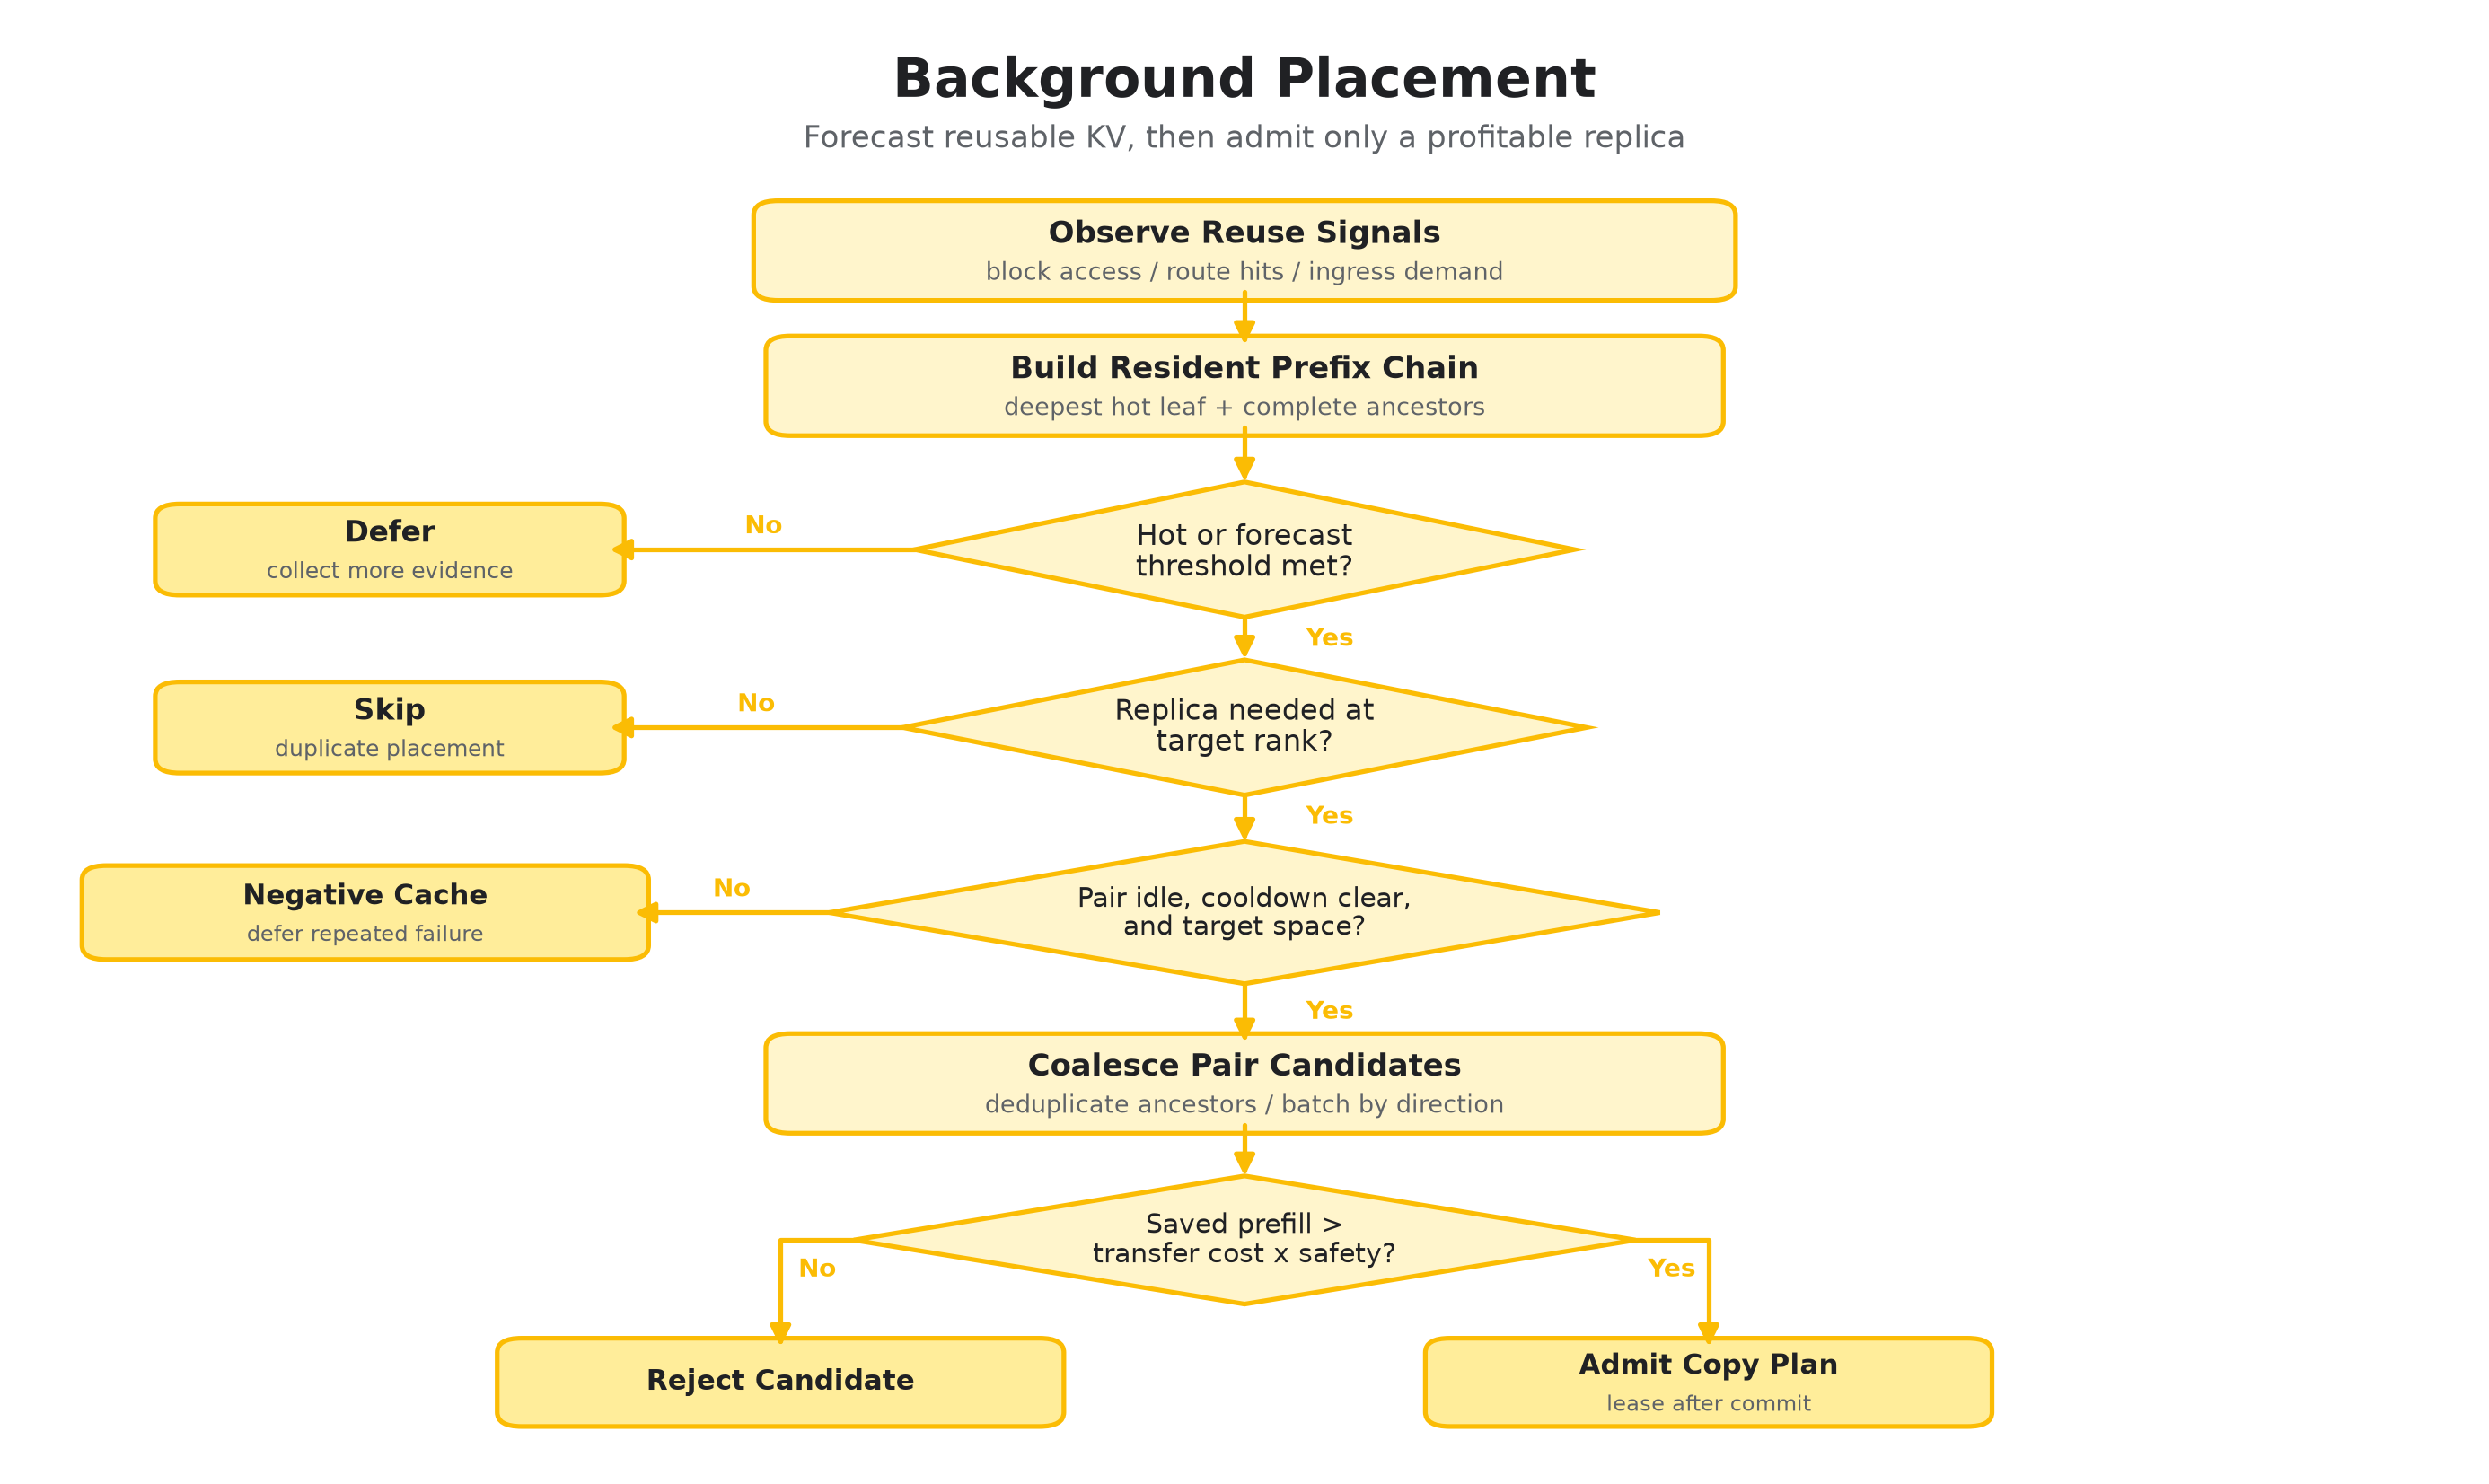
\includegraphics[width=0.9\textwidth]{fig_hot_prefix_decision.png}
  \caption{Background-placement decision. Complete-block observations and ingress forecasts create candidates, but replica need, load/placement conditions, cooldown, pair idleness, target capacity, and measured benefit remain mandatory gates.}
  \label{fig:hot-prefix-decision}
\end{figure*}

\begin{figure*}[t]
  \centering
  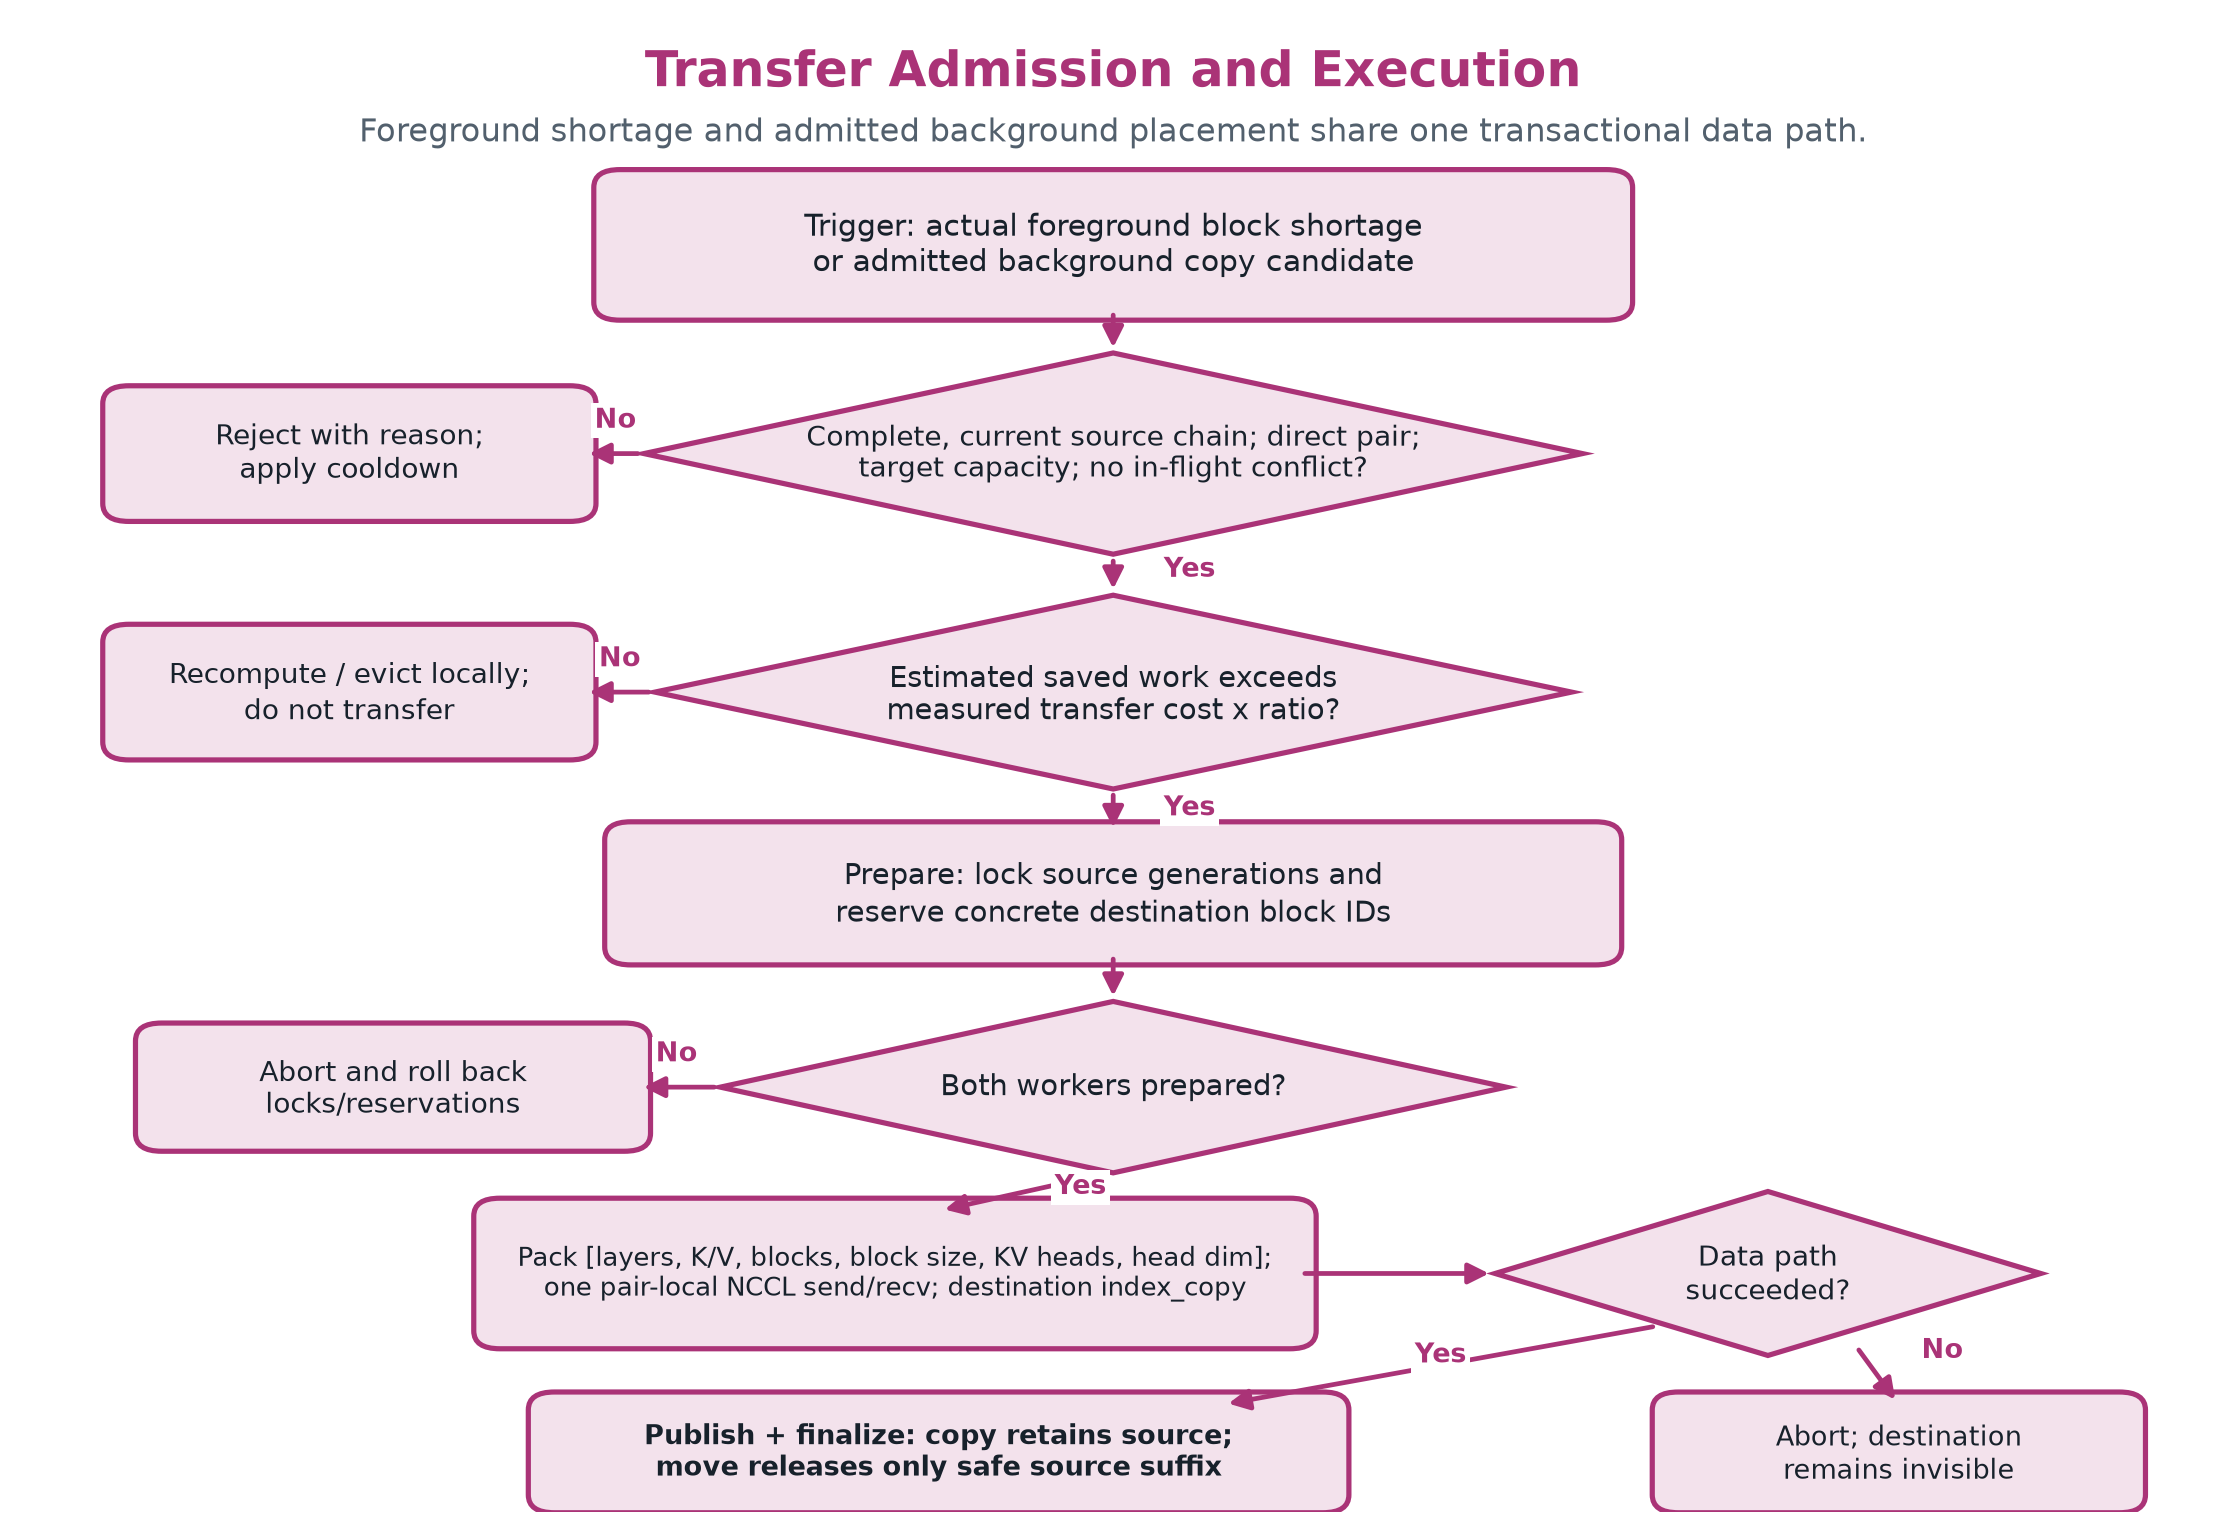
\includegraphics[width=0.9\textwidth]{fig_transfer_decision.png}
  \caption{Transactional transfer path. A foreground plan carries only an actual block shortage; a background plan carries an already admitted reusable chain. Both use the same source-validity and benefit checks, prepare, packed pair-local NCCL payload, publish/finalize, and abort path.}
  \label{fig:transfer-decision}
\end{figure*}

\subsection{Process and Ownership Model}

LLMEngine is the user-facing process. It creates one independent control-plane process and $N$ identical data-plane processes, including a worker for rank~0. New sequences enter LLMEngine, which sends sequence metadata and prefix hashes through a ControlPlaneClient. The control plane chooses a rank before LLMEngine enqueues the full sequence to that worker. Workers do not normally rerun global routing.

The control process owns GlobalScheduler and GlobalBlockManager. A data-plane process owns one Local Scheduler, Local Block Manager, Model Runner, and CUDA device. This separation is an ownership boundary: the global page table is authoritative metadata, whereas local block managers are authoritative for physical allocation, reference counts, readiness, and the KV tensor. Global Scheduler sends route targets and transfer phases to each Local Scheduler. Each Local Block Manager sends a versioned snapshot to Global Block Manager after a relevant state change. No Python BlockManager object is shared across processes.

Figure~\ref{fig:arch} distinguishes three communication classes. The request/result path carries full Sequence objects, generated tokens, and runtime measurements between LLMEngine and one selected worker. The metadata/control path carries versioned block and load snapshots upward and transfer phases plus heartbeat commands downward. The KV data path bypasses both processes: the source Model Runner gathers a contiguous tensor from its local HBM cache, the pair-local NCCL communicator carries it over direct NVLink, and the destination Model Runner scatters it into blocks reserved by its own Local Block Manager.

LLMEngine also monitors the control process and can restart it. Bidirectional heartbeat messages detect an unresponsive worker or control process; they provide failure detection, not consensus or high availability. Worker state snapshots reconstruct control metadata after a control-process restart. The current prototype does not continue service after launcher failure.

\subsection{Authoritative Global Metadata}

GlobalBlockManager maintains a page table $h \mapsto \{(g,b,\mathrm{generation},\mathrm{ready})\}$ that may contain multiple replicas for one hash. It also stores versioned free, used, evictable, parent, recency, and access-frequency snapshots per GPU, together with route reservations, in-flight transfer blocks, placement leases, worker epochs, and snapshot versions used to reject stale updates.

Workers publish a complete snapshot after allocation, append, release, preemption, transfer publication, and relevant cache-access changes. Replacement is atomic at GPU-snapshot granularity. Route-time reservations optimistically subtract capacity until the request commits its first prefill, preventing a burst of routes from all consuming the same stale free-block count. A heartbeat never advances page-table freshness; missing or stale snapshots trigger an explicit full-state request.

\subsection{KV-Aware Routing}
\label{sec:routing}

For a request initially assigned to rank $s$, candidate ranks are $s$ and its directly connected NVLink partners. The topology affinity is
\begin{equation}
 w(s,g)=
 \begin{cases}
 2, & g=s,\\
 1, & g\text{ is directly connected to }s\text{ by NVLink},\\
 0, & \text{otherwise}.
 \end{cases}
\end{equation}
The zero case is filtered rather than carried into later scoring.

For candidate rank $g$, let $N$ be prompt tokens, $R$ request blocks, $h_g$ the longest contiguous ready-prefix match, $S$ the block size, and $F_g$ the current free blocks. The required new blocks, uncached prefill work, and reclaim pressure are
\begin{align}
 n_g &= \max(0,R-h_g), \\
 M_g &= \min(N,n_gS), \\
 A_g &= \max(0,n_g-F_g).
\end{align}
A rank is feasible only when its free plus dependency-safe reclaimable capacity covers $n_g$. Its token-equivalent queue work is
\begin{equation}
 Q_g = w_w(T_g^{\mathrm{wait}}+T_g^{\mathrm{pending}})
     + w_rT_g^{\mathrm{running}}
     + w_s(N_g^{\mathrm{running}}+N_g^{\mathrm{pending}}),
\end{equation}
with current defaults $w_w=1$, $w_r=0.25$, and $w_s=32$. GlobalScheduler then minimizes
\begin{equation}
 C_{\mathrm{route}}(g) = Q_g + w_pM_g + w_eA_gS,
\end{equation}
where $w_p=1$ and $w_e=0.5$ by default. Thus locality enters through $h_g$ and directly removes missing prefill work; it is not an independent hit-rate reward subtracted from cost. Prefix/topology score breaks equivalent-cost ties.

\begin{figure*}[t]
  \centering
  
\includegraphics[width=0.96\textwidth]{fig_routing_cost_model.png}
  \caption{Routing cost model. Each capacity-feasible rank is priced by token-aware queued work, uncached prefill implied by its contiguous prefix match, and dependency-safe reclaim pressure. A bounded spill is allowed only when the prefix owner is sufficiently more loaded and the additional recomputation cost remains within the configured bound.}
  \label{fig:routing-cost-model}
\end{figure*}

The lowest-cost feasible candidate wins. A prefix owner may be bypassed when its sequence pressure exceeds that of a lower-pressure rank by a configured threshold and the extra recomputation cost remains bounded. On a miss, the router chooses the lowest projected-cost rank with sufficient effective capacity. This policy controls request/load skew and replica underutilization; it does not change the underlying data-parallel execution strategy.

\subsection{Local Allocation and Reclamation}

The Local Block Manager first references a matching ready local block and increments its reference count. Otherwise, it allocates from a deque of free block identifiers and publishes a complete block only after the model has written its KV data. Completed prefixes remain cacheable at reference count zero. Reclamation operates on dependency-safe leaves so removing an ancestor cannot orphan a retained descendant. Coldness combines access frequency and recency; live blocks with positive references are not move-eviction victims, although they may be copied when replication is profitable. Figure~\ref{fig:kv-block-lifecycle} summarizes both the normal local path and the transactional cross-GPU branch.

\begin{figure*}[t]
  \centering
  
\includegraphics[width=0.98\textwidth]{fig_kv_block_lifecycle.png}
  \caption{KV-block lifecycle. The Local Block Manager owns allocation, generation, readiness, reference, and cache state; ModelRunner writes or transfers the physical K/V tensor. A complete block with \texttt{ref\_count=0} remains cached until a hit or dependency-safe reclaim. During transfer, reserved and received-but-unpublished destination blocks remain invisible to routing. Publication precedes copy/move finalization, and abort restores the source while freeing the destination reservation.}
  \label{fig:kv-block-lifecycle}
\end{figure*}

The separation between ``received'' and ``published'' is the visibility boundary. A successful NCCL receive alone does not create a routable replica: the destination first records the complete hash chain and readiness in its local snapshot, after which the control plane may expose that location. For copy semantics, a referenced source remains valid and is merely unlocked. For move semantics, only an unreferenced dependency-safe suffix is reclaimed. Partial or not-yet-ready local blocks bypass the cache and return directly to the free deque when released.

\subsection{Foreground Transfer}
\label{sec:fg-transfer}

Foreground transfer is demand-driven. If a local prefill or decode append has a shortage of $k$ blocks, the worker asks the control plane for exactly $k$, not for the request's full block count. GlobalScheduler selects a complete source chain and determines whether the operation is a move or a copy. A move may release a dependency-safe source suffix after publication; a copy retains the source and creates another replica. Pinned prefixes can be copied but never released.

For $B$ blocks, $L$ layers, block size $S$, $H_{kv}$ KV heads, head dimension $D$, and $d$ bytes per element, the packed payload is $X=2BLSH_{kv}Dd$. For each logical NVLink pair $p$, the transfer microbenchmark supplies monotonic P95 samples $\{(X_i,Q^{95}_{p,i})\}$. The data-path prior and static estimate are
\begin{align}
 T_{\mathrm{data}}^{p}(X) &= \operatorname{PWL}\!\left(X;\{(X_i,Q^{95}_{p,i})\}\right), \\
 T_{\mathrm{static}}^{p}(X) &= (T_{\mathrm{fixed}}+I T_{\mathrm{data}}^{p}(X))w_x.
\end{align}
Interpolation is linear between adjacent samples; plans outside the measured range use the nearest boundary or the final measured slope. Let $b(B)=2^{\lceil\log_2 B\rceil}$ be the size bucket. Completed source operations and dispatch-to-publication observations update separate nonnegative residual EWMAs $\Delta^{src}_{p,b}$ and $\Delta^{place}_{p,b}$. Admission remains conservative:
\begin{equation}
 T_{\mathrm{xfer}}=\max\!\left(
 T_{\mathrm{static}}^{p},
 (T_{\mathrm{data}}^{p}+\Delta^{src}_{p,b})w_x,
 (T_{\mathrm{fixed}}+I T_{\mathrm{data}}^{p}+\Delta^{place}_{p,b})w_x
 \right).
\end{equation}
The paper configuration uses $T_{\mathrm{fixed}}=40$ ms and $I=1.2$.
These values are not inferred from idle bandwidth alone: a separate
Qwen3-0.6B serving pilot measured complete target-side transactions for short
foreground plans. Subtracting the same-size profile term left a 32--38 ms
per-plan residual, rounded upward to 40 ms. Modeling this residual additively
fits both short foreground and large coalesced handoff plans better than
multiplying every payload by the short-plan slowdown.
Foreground saved work uses discounted historical chain reuse $\widehat{R}$, whereas background admission counts only the first avoidable cold prefill because the destination self-warms after a miss:
\begin{align}
 T_{\mathrm{save}}^{fg} &= \widehat{R}BS t_{\mathrm{prefill}}, \\
 T_{\mathrm{save}}^{bg} &= BS t_{\mathrm{prefill}}(g_{dst}).
\end{align}
A plan is admitted only if source generations and target capacity are valid and $T_{\mathrm{save}} \ge \rho T_{\mathrm{xfer}}$ for the configured safety ratio $\rho$. Repeated identical low-benefit or no-space background candidates enter the negative cache until their signature changes.

\begin{figure*}[t]
  \centering
  
\includegraphics[width=0.96\textwidth]{fig_transfer_cost_model.png}
  \caption{Transfer cost and benefit model. Payload geometry indexes a measured pair-specific P95 latency curve; source and dispatch-to-publication residuals are learned independently per pair and size bucket. Foreground and background paths use different saved-work estimates but share validity, capacity, and benefit-ratio gates.}
  \label{fig:transfer-cost-model}
\end{figure*}

\subsection{Background Placement}
\label{sec:bg-transfer}

Background placement handles predictable future reuse rather than an immediate allocation failure. Workers report cumulative access counts and parent hashes for ready blocks; the control plane selects maximal chains by their deepest hot leaf and restores all resident ancestors in prefix order. Route-hit counts provide an online trigger. When ingress knows queued but not-yet-submitted requests, it may additionally provide a hash-to-demand forecast; the session-handoff benchmark uses this explicit signal. Predicted reuse is capped future demand when available, otherwise the minimum chain access count minus its already-observed use, discounted conservatively. This signal only creates a candidate. The destination must still lack the replica, the directed pair must clear cooldown and idle-pressure checks, and the target must have space.

Compatible candidates are deduplicated and batched by directed NVLink pair. The current defaults cap one candidate chain at eight blocks and the coalesced pair payload at 128 blocks; these are upper bounds rather than a fixed transfer size. Admission counts at most the first avoidable cold prefill at the destination, because without an intervening eviction that GPU would self-warm after its first miss; it does not multiply benefit by every forecast request. A placement lease is created only after publication. Its explicit source and replica quotas stripe later matching requests across both GPUs, coupling speculative placement to routing rather than merely duplicating data.

The session-handoff workload exercises this path: a warmup phase creates one copy of each long prefix, then a reuse phase shifts sessions to the partner. The locality and load-skew workloads can deliberately disable background placement to isolate routing and steady-state overhead.

\subsection{Transactional Transfer Protocol}

A plan has four externally visible phases. During prepare, the destination reserves concrete free block IDs and both workers record plan state; no new location is visible to routing. During execute, source and destination issue matching NCCL point-to-point operations. The source gathers physical blocks with index selection into one contiguous tensor of shape $[L,2,B,S,H_{kv},D]$, representing layers, K/V, transferred blocks, block tokens, KV heads, and head dimension. It sends that tensor once on a prewarmed pair-specific process group; the destination receives an equal-shaped buffer and scatters it into reserved physical blocks with indexed copies. Hashes, generations, and destination block IDs remain control-protocol metadata rather than part of the NCCL tensor payload. During publish, the destination marks received blocks ready and publishes a versioned snapshot. Only then may the control plane expose the new page-table location or lease. During finalize, a move verifies the source block hash and generation before releasing the specified suffix, whereas a copy retains the source. A prepare or execute failure aborts the transaction, releases reservations, and keeps the source authoritative.

The protocol is idempotent by plan ID and phase. Per-client receive locks serialize response-queue consumption, control-plane state is mutated in one event loop, and local block mutations remain single-threaded inside a worker. These measures avoid a global lock on the inference fast path while protecting metadata transactions.

\section{Implementation}
\label{sec:impl}

\sys{} extends Mini-vLLM in Python and PyTorch. Table~\ref{tab:modules} summarizes the implementation boundaries. Legacy function names swap\_out and swap\_in remain inside the KV-transfer module; the paper and public documentation use transfer because the data path supports both copies and moves and is not a CPU swap tier.

\begin{table}[t]
  \centering
  \caption{Principal implementation modules.}
  \label{tab:modules}
  \footnotesize
  \setlength{\tabcolsep}{3.5pt}
  \begin{tabular}{@{}L{0.34\linewidth}L{0.60\linewidth}@{}}
    \toprule
    Module & Responsibility \\
    \midrule
    LLM engine & Ingress, process launch/supervision, completion aggregation \\
    Control plane & Protocol, clients, authoritative event loop, heartbeat \\
    Global scheduler & Route and transfer-plan cost decisions \\
    Global block manager & Global page table, snapshots, reservations, candidates \\
    Data plane & Per-rank worker loop and transfer phase executor \\
    Local scheduler & Local prefill/decode admission and shortage trigger \\
    Local block manager & Physical blocks, prefix cache, references, reclamation \\
    Model runner & Model execution, KV tensor, metrics, transfer entry \\
    KV transfer & Packed NCCL GPU-to-GPU payload movement \\
    \bottomrule
  \end{tabular}
\end{table}

\subsection{Testing Strategy}

The repository mirrors each engine module with focused tests rather than relying only on benchmark completion. The current CPU test run contains 190 passing tests and one hardware-gated skip. Table~\ref{tab:tests} lists the coverage intent.

\begin{table}[t]
  \centering
  \caption{Test design and coverage.}
  \label{tab:tests}
  \footnotesize
  \setlength{\tabcolsep}{3.5pt}
  \begin{tabular}{@{}p{0.30\linewidth}p{0.62\linewidth}@{}}
    \toprule
    Test group & Covered behavior \\
    \midrule
    Block managers & Allocation/release, chain reuse, LFU/LRU leaves, generations, snapshots \\
    Global scheduler & Hit/miss/capacity routes, load bypass, direct-pair filtering, move/copy plans \\
    Control plane & Epochs, stale updates, reservations, leases, idempotent phases, heartbeat, concurrency \\
    Data plane/engine & Queue protocol, master-first ingress, worker/control lifecycle, aggregation \\
    KV transfer & Shape/byte accounting, copy/move primitives, two-rank NCCL equality and deadlock guard \\
    Model runner & KV layout, prefill/decode preparation, dtype consistency, transfer adapters \\
    Benchmarks & Workloads, schemas, metrics, confidence intervals, plotting, transfer-profile construction and validation \\
    End-to-end & Multi-process request completion and optional CUDA/NCCL integration \\
    \bottomrule
  \end{tabular}
\end{table}

Tests use fakes for deterministic control decisions and mark CUDA/NCCL cases so CPU-only CI remains usable. The hardware test sends known KV values from rank~0 to rank~1, verifies equality after transfer, and bounds completion to detect mismatched send/receive ordering.

\section{Evaluation}
\label{sec:eval}

We answer four questions: (Q1) Does KV-aware routing improve useful prefix reuse? (Q2) What latency and bandwidth does the transfer data path provide? (Q3) Does combining routing and transfer improve end-to-end service when sessions move? (Q4) Under which skew workloads does transfer fail to amortize its cost?

\subsection{Setup and Methodology}

The evaluation uses six 24~GiB GeForce RTX 3090 GPUs selected from a seven-GPU host. Physical pairs $(0,1)$, $(3,4)$, and $(5,6)$ report NV4 connectivity; the processes see them as logical pairs $(0,1)$, $(2,3)$, and $(4,5)$. We evaluate Qwen3-0.6B and Qwen3-1.7B in BF16. Both models have 28 layers, eight KV heads, head dimension 128, and therefore the same 114,688 KV bytes per token. The KV block size is 256 tokens. System experiments use a fixed per-worker KV block budget and five repetitions with seed~0 and EOS ignored, so every request produces 64 output tokens. Goodput counts output tokens from requests whose E2E latency is at most 10~s.

Every JSON artifact records the command, resolved model/configuration, Git state, per-trial values, 95\% confidence intervals, and per-rank statistics. Scenarios run in fresh processes; cache contents do not persist between them. The full artifact set is the paper batch dated 20260725T031840Z.

\subsection{Synthetic Dataset Profiling}

The current study uses deterministic synthetic prompts, not a public conversational trace. Each prompt applies the Qwen chat template to a repeated instruction body and group-specific suffix. This makes the amount and ownership of reusable KV explicit. Table~\ref{tab:datasets} profiles the tokenized inputs and phase construction. Dataset-level reporting is important because request hit rate alone hides how many prompt tokens are actually reusable.

We therefore report two intrinsic trace metrics before running any system policy. Let $m_i$ be the number of complete, contiguous prefix blocks of request $i$ whose cumulative hashes appeared in an earlier request, $B$ the block size, and $T_i$ the prompt length. Request prefix sharing is $\sum_i \mathbb{1}[m_i>0]/N$, while token prefix sharing is $B\sum_i m_i/\sum_i T_i$. These are ordered-replay upper bounds with unlimited cache and perfect placement; partial tail blocks are excluded. Runtime request hits and cached-token ratio are reported separately.

\begin{table*}[t]
  \centering
  \caption{Synthetic workload dataset profiles. Prompt-token counts and block-aligned sharing upper bounds are identical across the two Qwen3 tokenizers. Every request produces 64 output tokens in the paper runs.}
  \label{tab:datasets}
  \footnotesize
  \setlength{\tabcolsep}{3pt}
  \begin{tabular}{@{}L{0.10\textwidth}rL{0.23\textwidth}rrrrL{0.22\textwidth}@{}}
    \toprule
    Workload & Requests & Exact prefix construction & Prompt tokens & Req. share & Token share & Window & Phase construction and purpose \\
    \midrule
    Locality/routing & 192 & 16 recurring long-prefix groups; 12 requests per group & 365,880 & 91.67\% & 86.20\% & 16 & Seeded interleaving isolates locality-aware routing with transfer disabled. \\
    Load skew & 192 & 1 long hot group with 144 requests; 4 shorter recurring cold groups with 12 requests each & 320,232 & 97.40\% & 90.57\% & 16 & The 75\% hot family tests load pricing at a cache-owner hotspot. \\
    Memory skew & 128 & 15 reusable long hot groups; 32 shorter one-shot pressure prefixes & 214,064 & 63.28\% & 67.81\% & 16 & 32 warm-up, 32 pressure, and 64 reuse requests induce foreground shortage. \\
    Session handoff & 128 & 32 session-prefix groups; 1 warm-up and 3 reuse requests per group & 244,048 & 75.00\% & 70.49\% & 64 & 32 source warm-ups and 96 partner-side reuses test predictive placement. \\
    \bottomrule
  \end{tabular}
\end{table*}

\subsection{Baselines and Metrics}

We use five normalized scenarios. The single-gpu scenario runs one replica. The multi-gpu scenario uses static round-robin data parallelism. The multi-gpu-kv-routing scenario enables the global router but disables transfer. The multi-gpu-kv-transfer scenario keeps round-robin request placement and enables transfer. The multi-gpu-lmpool scenario enables both mechanisms. All multi-GPU scenarios use the same per-worker KV block budget.

Primary metrics are output throughput, SLA goodput, mean TTFT, mean time per output token (TTPT), mean and P90 E2E latency, and uncached prefill tokens. We distinguish control-plane request hit, route-to-owner hit, data-plane local request hit, and cached-token ratio. Transfer counters report blocks, bytes, copy/move semantics, protocol success/failure, and estimated versus observed cost. Per-rank request/token/time/utilization distributions expose load concentration.

Figure~\ref{fig:results-summary} summarizes three distinct claims. Panel~(a) compares cached prompt tokens under round-robin and KV-aware routing. Panel~(b) plots mean measured NVLink bandwidth over plan sizes from one to 64 blocks; the shaded band spans the minimum and maximum over two models and three physical pairs and is not a confidence interval. Panel~(c) reports the improvement of full \sys{} over multi-gpu in session handoff; positive bars denote either higher throughput or lower latency.

\begin{figure*}[t]
  \centering
  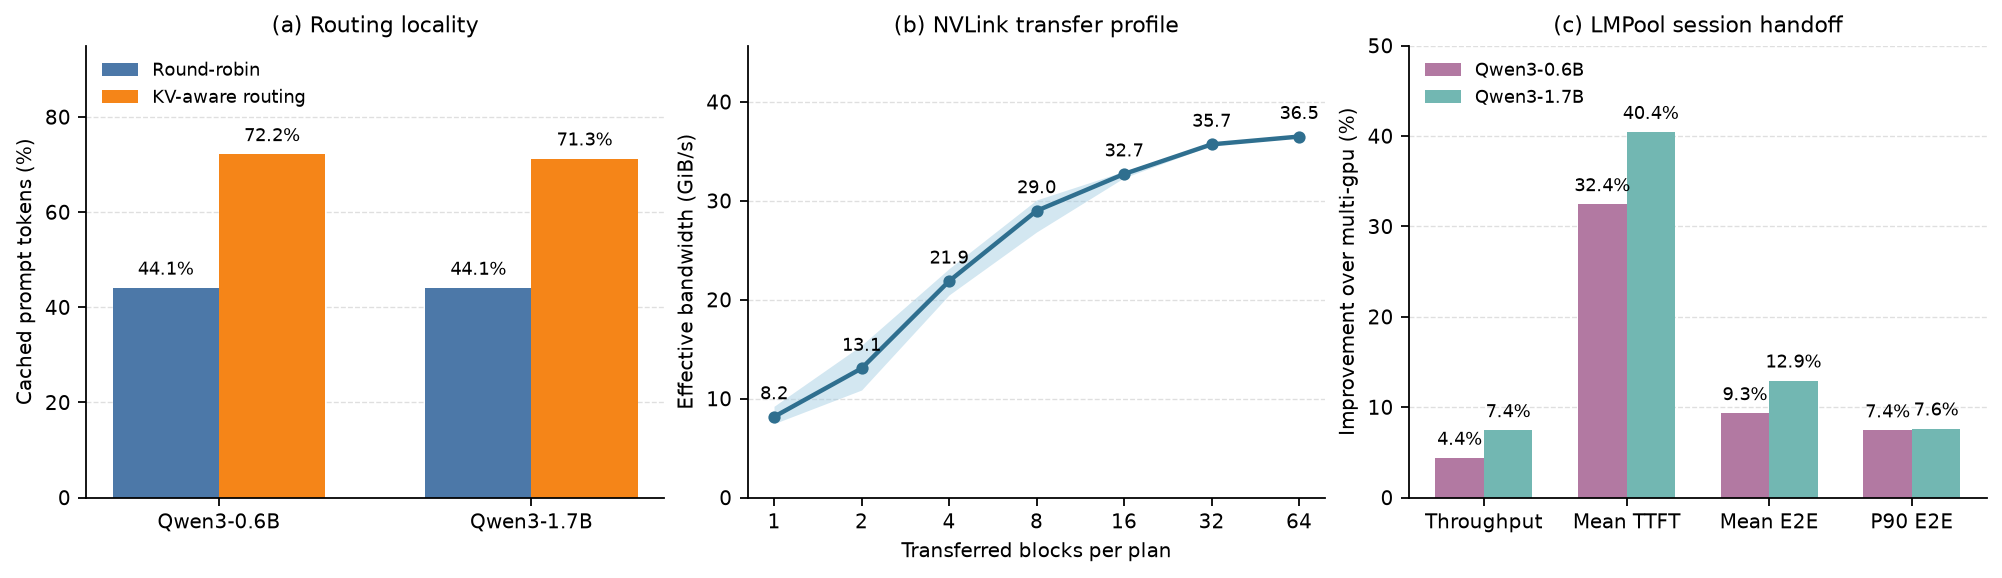
\includegraphics[width=\textwidth]{fig_results_summary.png}
  \caption{Summary of locality, transfer-data-path, and end-to-end session-handoff results. End-to-end values are five-trial means. The transfer line is the mean over six model/pair runs, and its shaded band is their observed minimum--maximum range. Numeric labels make the plots interpretable without relying only on color.}
  \label{fig:results-summary}
\end{figure*}

Figure~\ref{fig:absolute-results} retains the original units for the two workloads behind the main claims. Routing keeps throughput close to round-robin while increasing useful token reuse; its TTFT effect is model-dependent. Full \sys{} has the highest session-handoff throughput and the lowest TTFT for both models. The complete benchmark outputs, including E2E tails, reuse, and GPU utilization, are retained with the archived artifact and the accompanying technical report.

\begin{figure*}[t]
  \centering
  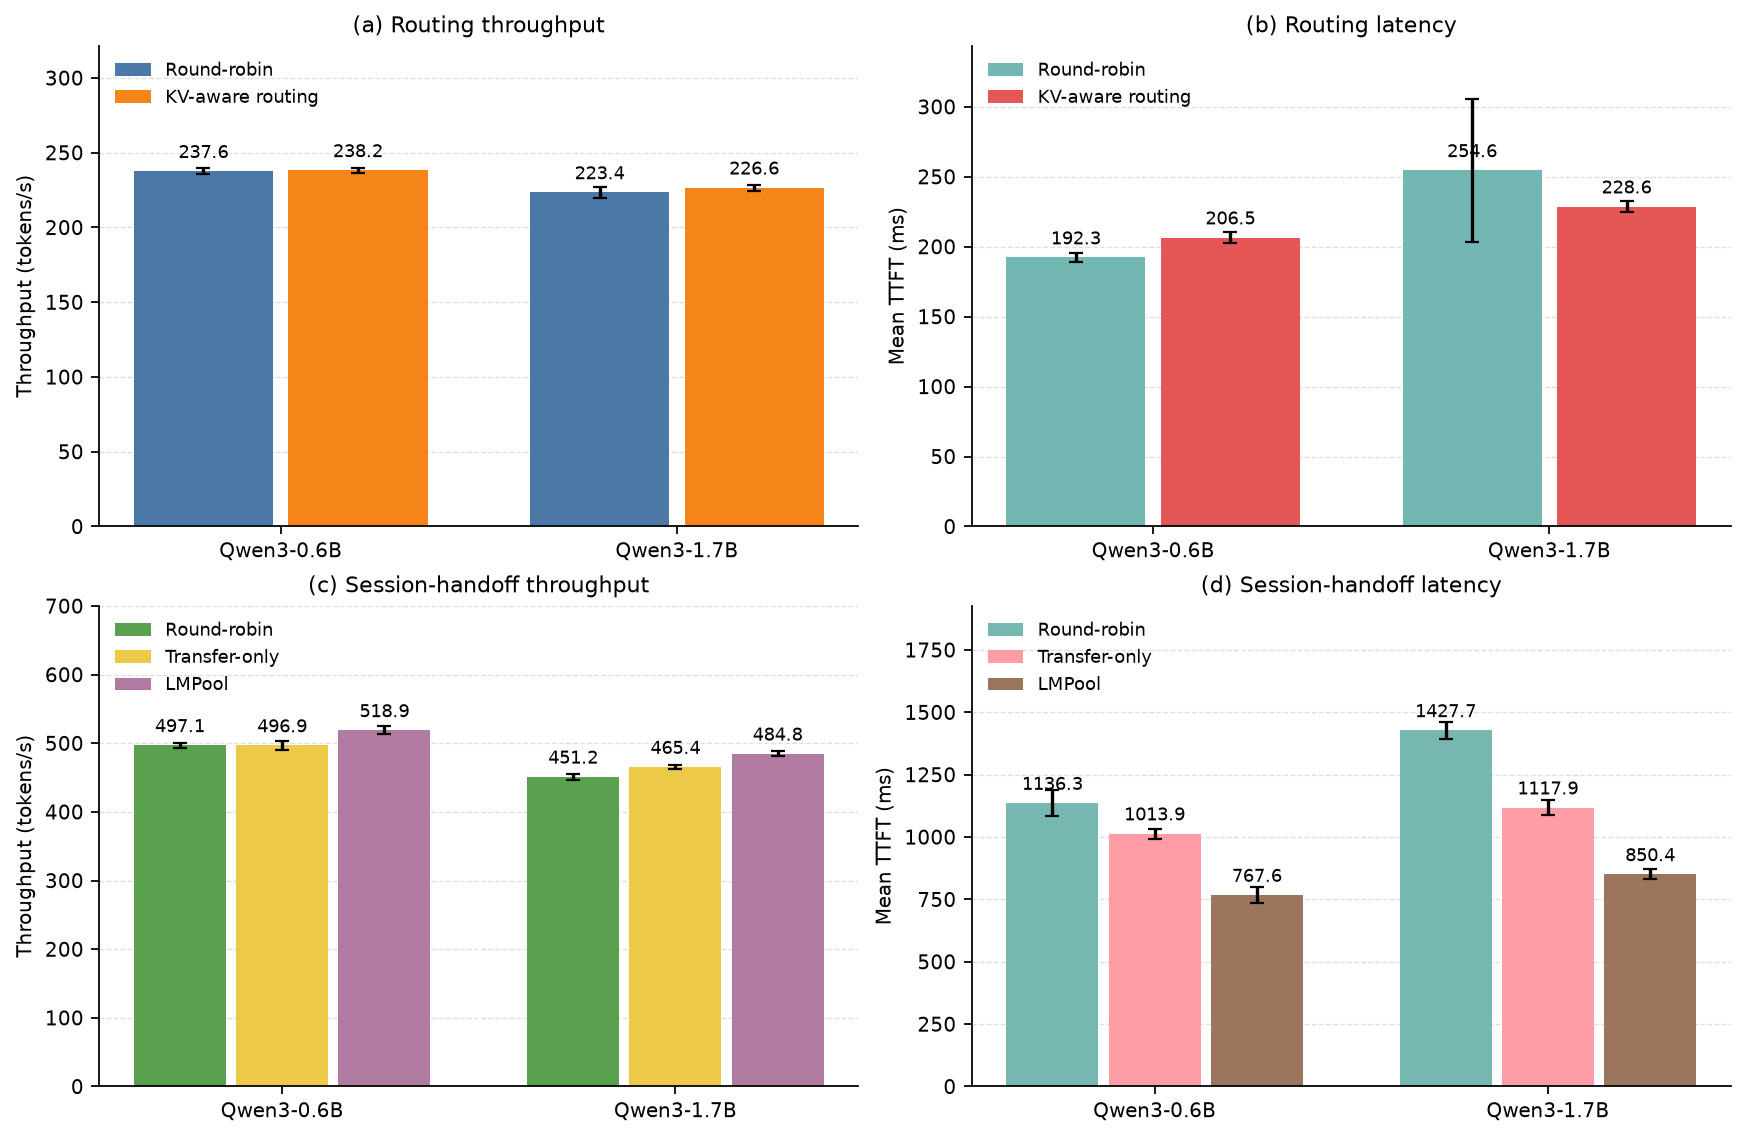
\includegraphics[width=\textwidth]{fig_absolute_metrics.png}
  \caption{Absolute five-trial mean results in their original units. Panels (a)--(b) show throughput and mean TTFT for the locality/routing workload, comparing round-robin with KV-aware routing under the same KV budget. Panels (c)--(d) show the session-handoff workload, comparing round-robin, transfer-only, and full \sys{}. Numeric labels report each model's mean, and error bars show 95\% confidence intervals. The archived benchmark figures retain the wider metric set.}
  \label{fig:absolute-results}
\end{figure*}

\subsection{Q1: Routing Improves Token Reuse}

Table~\ref{tab:routing} compares routing-only with round-robin. Cached-token ratio rises from 44.1\% to 72.2\% on Qwen3-0.6B and from 44.1\% to 71.3\% on Qwen3-1.7B. Uncached prefill tokens fall by 50.2\% and 48.6\%, respectively. The prompts and KV budget are unchanged, so this difference comes from placement rather than extra cache capacity. Throughput changes by only 0.2\% on Qwen3-0.6B and 1.4\% on Qwen3-1.7B, both small relative to run-to-run variation. Mean TTFT increases by 7.4\% on Qwen3-0.6B but decreases by 10.2\% on Qwen3-1.7B. These results establish that routing finds and realizes more reusable KV; they do not support a universal latency improvement for this workload.

\begin{table}[t]
  \centering
  \caption{Routing workload, five-trial means. Uncached is the total prompt tokens actually prefetched.}
  \label{tab:routing}
  \footnotesize
  \setlength{\tabcolsep}{3.2pt}
  \begin{tabular}{@{}llrrrr@{}}
    \toprule
    Model & Policy & Tok/s & TTFT (ms) & Cached & Uncached \\
    \midrule
    0.6B & Round-robin & 237.6 & 192.3 & 44.1\% & 204,549 \\
         & Routing & 238.2 & 206.5 & 72.2\% & 101,842 \\
    1.7B & Round-robin & 223.4 & 254.6 & 44.1\% & 204,651 \\
         & Routing & 226.6 & 228.6 & 71.3\% & 105,170 \\
    \bottomrule
  \end{tabular}
\end{table}

\subsection{Q2: Batched NVLink Transfer}

The microbenchmark moves every layer's K and V tensors between two ranks and validates the destination byte-for-byte. It checks the packed tensor shape, byte count, dtype path, and receive-side contents; measures pair- and plan-size-specific latency and effective bandwidth; and supplies the P95 samples used to initialize the online transfer-cost model. It does not establish end-to-end serving benefit, which also depends on future reuse and interference.

Four blocks contain 0.109~GiB and achieve 20.5--23.1~GiB/s across all model/pair runs, with 4.73--5.34~ms mean latency. Eight blocks contain 0.219~GiB and achieve 26.8--30.1~GiB/s with 7.27--8.15~ms mean latency. Mean bandwidth reaches 36.5~GiB/s at 64 blocks. Larger batches better amortize fixed NCCL and kernel overhead. Because the two Qwen3 models have identical KV geometry, their payload sizes are identical; running both checks model resolution and dtype paths rather than creating a different transfer size.

These values are samples on the online latency profile, not fixed runtime transfer sizes. Foreground plans follow the actual shortage, and background plans can coalesce several chains on one directed pair. The experiment measures 1/2/4/8/16/32/64 blocks on every physical pair, constructs a logical-pair P95 piecewise-linear profile, and then updates pair-by-size-bucket residuals from completed serving transfers. A useful plan must still save more prefill time than this measured latency plus runtime interference.

\subsection{Q3: Session Handoff Benefits from Both Principles}

Table~\ref{tab:handoff} reports the strongest end-to-end case. After 32 warmup sessions, \sys{} copies 224 hot blocks per trial in three batched pair plans, then routes the 96 reuse requests across source and replica. Cached-token ratio rises from 47.0\% under round-robin to 70.5\%. Compared with multi-gpu, full \sys{} improves throughput by 4.4\% on 0.6B and 7.4\% on 1.7B; mean TTFT falls by 32.4\% and 40.4\%; mean E2E falls by 9.3\% and 12.9\%. Transfer-only reduces TTFT for both models, while routing plus placement gives the highest throughput and lowest mean TTFT and E2E. The per-rank submitted-request max/min ratio falls from 3.3 to 1.8, showing that replication preserves locality without concentrating all reuse at the original owner.

\begin{table*}[t]
  \centering
  \caption{Session-handoff results, five-trial means. Parentheses show change relative to multi-gpu for the same model.}
  \label{tab:handoff}
  \footnotesize
  \setlength{\tabcolsep}{5pt}
  \begin{tabular}{@{}llrrrrrr@{}}
    \toprule
    Model & Policy & Throughput & Mean TTFT & Mean E2E & P90 E2E & Cached tokens & Blocks copied \\
          &        & (tok/s) & (ms) & (ms) & (ms) & & \\
    \midrule
    0.6B & Multi-gpu & 497.1 & 1,136.3 & 5,515.1 & 6,251.0 & 47.0\% & 0 \\
         & Transfer-only & 496.9 (-0.05\%) & 1,013.9 (-10.8\%) & 5,424.8 (-1.6\%) & 6,128.0 (-2.0\%) & 70.5\% & 224 \\
         & LMPool & 518.9 (+4.4\%) & 767.6 (-32.4\%) & 5,001.1 (-9.3\%) & 5,787.1 (-7.4\%) & 70.5\% & 224 \\
    \midrule
    1.7B & Multi-gpu & 451.2 & 1,427.7 & 6,121.4 & 7,039.5 & 47.0\% & 0 \\
         & Transfer-only & 465.4 (+3.2\%) & 1,117.9 (-21.7\%) & 5,746.1 (-6.1\%) & 6,554.0 (-6.9\%) & 70.5\% & 224 \\
         & LMPool & 484.8 (+7.4\%) & 850.4 (-40.4\%) & 5,329.7 (-12.9\%) & 6,502.5 (-7.6\%) & 70.5\% & 224 \\
    \bottomrule
  \end{tabular}
\end{table*}

\subsection{Q4: Boundary Results}

The memory-skew workload does not produce a transfer-dominated win. With Qwen3-1.7B, multi-gpu reaches 216.3 tok/s, transfer-only 212.6 tok/s, and full \sys{} 214.5 tok/s. No transfer is admitted for this model. Full \sys{} reduces mean TTFT from 469.8 to 407.8~ms and mean E2E from 4,572.7 to 4,505.4~ms, but throughput remains lower and P90 E2E changes little. Qwen3-0.6B admits seven copied blocks in only one of five trials; averaged over all trials, full \sys{} records one copied block and also loses throughput. The baseline therefore has little pathological work for transfer to remove. This is evidence that admission suppresses unprofitable movement, not a broad performance claim.

Under steady load skew, no transfers are admitted and all multi-GPU policies remain within 0.6\% throughput of round-robin. This is a useful control: \sys{} does not manufacture data movement when placement is already adequate, but its control and routing overhead is not free. We therefore use locality to substantiate reusable-KV placement, the microbenchmark to substantiate the data path and its cost prior, and session handoff to substantiate their composition. Memory and load skew define the current prototype's limits rather than universal wins.

\section{Discussion and Limitations}
\label{sec:limitations}

The synthetic phase structure makes causal attribution possible, but it is not a substitute for profiling production traces. Future evaluation should replay a published or anonymized trace and report prefix popularity, reuse distance, prompt/decode distributions, and session-affinity transitions before selecting cache policies.

The study uses one host, six consumer GPUs, and two sub-2B models with identical KV geometry. Larger models change the compute-to-transfer ratio, and larger NVLink fabrics change candidate selection. Results should not be extrapolated to RDMA or PCIe-only clusters.

Versioned snapshots, transactional transfers, heartbeats, and launcher restart protect consistency and detect failures. They do not implement replicated consensus; launcher failure stops the service and a worker failure may lose its physical cache.

The model- and pair-specific size curve, calibrated fixed transaction residual, and bucketed EWMA capture payload scale and observed serving overhead, but they do not explicitly condition on concurrent kernels, clocks, or link contention. Rapidly changing compute states can therefore still be mispriced; a production implementation should add concurrency-aware features after collecting enough serving samples.

\section{Related Work}
\label{sec:related}

\subsection{LLM Serving and Prefix Caching}

Orca introduced iteration-level scheduling for transformer serving~\citep{ORCA}. vLLM's PagedAttention virtualizes KV allocation into blocks~\citep{vLLM}, while SGLang's RadixAttention organizes reusable prefix state for structured programs~\citep{SGLang}. Sarathi-Serve uses chunked prefill to control prefill/decode interference~\citep{SarathiServe}; DistServe separates the two phases and optimizes goodput under TTFT and TPOT constraints~\citep{DistServe}. These systems establish the local execution and scheduling context. \sys{} instead studies admission-time placement among data-parallel replicas whose KV blocks can be copied over direct NVLink.

\subsection{Distributed and Tiered KV Caches}

Mooncake introduced a KV-cache-centric disaggregated architecture that trades distributed storage for prefill computation~\citep{Mooncake}. The newer vLLM--Mooncake Store integration pools KV across instances through GPUDirect RDMA and a distributed DRAM/SSD service. Its official agentic-trace evaluation reports 3.8$\times$ throughput, 46$\times$ lower P50 TTFT, and 8.6$\times$ lower E2E latency on 12 GB200 GPUs; a synthetic scale-out experiment maintains over 95\% cache hits at 60 GPUs~\citep{MooncakeStore}. The integration can query block hashes during scheduling, while its authors list full cache-aware routing and multi-node NVLink as future work. PegaFlow instead moves cache ownership into a long-lived Rust service and combines pinned host DRAM, one-sided RDMA reads, and local SSD. The vLLM/Novita report shows 56\% higher throughput from sharing one fixed host-cache budget across eight Qwen3-8B instances, 72\% for deduplicated TP8 MLA KV, and 194~GB/s average reads for at least 1-GiB objects on an eight-NIC RDMA cluster~\citep{PegaFlow}.

MemServe provides an elastic memory pool and global prompt-tree scheduler for disaggregated serving~\citep{MemServe}. CachedAttention retains multi-turn KV in a hierarchy and overlaps loading/saving with compute~\citep{CachedAttention}. CacheGen compresses KV for faster context loading over constrained links~\citep{CacheGen}, and LMCache exposes a reusable cache layer across engines and storage/communication backends~\citep{LMCache}. These systems emphasize capacity, persistence, or cross-node visibility. \sys{} deliberately addresses a narrower scale-up domain: physically local HBM caches on data-parallel replicas connected by direct NVLink.

\subsection{Migration and Multi-GPU Memory Balance}

Aqua uses spare memory on NVLink/NVSwitch-connected GPUs to page inference state for preemptive, time-sliced serving under bursty memory pressure. On eight H100 GPUs, it reports up to 20$\times$ better responsiveness and 4$\times$ higher throughput for a single long prompt~\citep{Aqua}. Aqua therefore provides fluidity for active inference state, but does not route requests by content-addressed prefix ownership. Llumnix migrates requests to support dynamic rescheduling and defragmentation~\citep{Llumnix}. MELL jointly considers multi-GPU KV load and request-migration cost~\citep{MELL}. Their work confirms that movement is a costed scheduling operation, not a universally beneficial fallback. \sys{} differs in using content-addressed prefix chains, copy-style replication, and placement leases to serve future requests from both source and destination.

Table~\ref{tab:related-principles} separates three concerns that are often grouped under ``distributed KV cache.'' Locality-aware placement sends a request where its prefix already exists. Fluidity-aware placement moves state when its current location is wrong. Coupled admission compares recomputation, queueing, capacity, and measured transfer cost before choosing between those actions. The comparison does not claim that \sys{} replaces durable or cross-node stores; it shows that \sys{} is the only listed design that closes all three decisions inside the serving scheduler.

\begin{table*}[t]
  \caption{Principle-oriented comparison of KV-cache systems. ``Partial'' denotes metadata lookup without a published joint locality/load routing and transfer-admission policy.}
  \label{tab:related-principles}
  \centering
  \small
  \setlength{\tabcolsep}{3pt}
  \begin{tabular}{L{0.12\textwidth}L{0.15\textwidth}L{0.17\textwidth}L{0.20\textwidth}L{0.12\textwidth}L{0.17\textwidth}}
    \toprule
    System & Primary scope & Locality-aware request placement & Fluidity mechanism and path & Durable / multi-tier pool & Coupled route--transfer admission \\
    \midrule
    Mooncake Store~\citep{MooncakeStore}
      & Cluster-wide agentic prefix reuse
      & Partial: hash lookup informs scheduling; full cache-aware routing is future work
      & Asynchronous GPUDirect RDMA between GPU HBM and distributed cache workers
      & Yes: DRAM and SSD
      & No published recompute-vs-transfer cost model \\
    PegaFlow~\citep{PegaFlow}
      & External, process-independent KV lifetime and sharing
      & No: vLLM retains request scheduling; a global index locates remote hits
      & CUDA IPC locally and one-sided RDMA across nodes; SSD for cold blocks
      & Yes: pinned DRAM, remote DRAM, SSD
      & No; TinyLFU governs cache admission, not route-vs-transfer choice \\
    Aqua~\citep{Aqua}
      & Responsive preemption under GPU-memory bursts
      & No content-addressed prefix routing
      & Inference-state paging to spare GPU HBM over NVLink/NVSwitch
      & No: volatile GPU HBM
      & Memory-pressure placement, not future prefix-reuse economics \\
    \sys{}
      & KV locality and fluidity across data-parallel GPU replicas
      & Yes: longest contiguous prefix jointly scored with load and effective capacity
      & Copy/move directly between peer HBM on configured NVLink pairs
      & No: volatile GPU HBM
      & Yes: route first, then admit transfer from measured cost and expected reuse \\
    \bottomrule
  \end{tabular}
\end{table*}

\section{Conclusion}
\label{sec:concl}

\sys{} coordinates physically local KV caches using two complementary principles: route first for cache locality, then transfer only when cache fluidity is worth its cost. The implementation separates an authoritative control process from per-GPU data processes, combines versioned metadata with transactional block movement, and limits cross-device decisions to direct NVLink pairs. Experiments show substantial reuse improvements from routing and cross-model TTFT/E2E gains for session handoff, while also showing that weak memory or load skew does not justify transfer. This boundary is central to the design: a useful KV pool is not one that moves the most data, but one that avoids recomputation and moves only data with measurable future value.

\section*{Acknowledgements}
Thanks to Yijun Sun and Prof. Kai Chen for project supervision, and to the Mini-vLLM authors for the base inference engine.

\bibliography{example_paper}
\bibliographystyle{mlsys2025}

\end{document}
